\documentclass[12pt, oneside]{article}

\setlength{\headheight}{14.49998pt}

\usepackage[spanish]{babel}
\usepackage{apacite}

\addto\captionsspanish{%
  \renewcommand{\tablename}{Tabla}
}

\usepackage[table,xcdraw]{xcolor}

\usepackage[T1]{fontenc}
% \usepackage{uarial}
% \renewcommand{\familydefault}{\sfdefault}

\usepackage{etoolbox}
\patchcmd{\thebibliography}{\section*{\refname}}{}{}{}


\usepackage{url}
\def\UrlBreaks{\do\/\do-}

\usepackage{adjustbox}
\usepackage{graphicx}
\usepackage{tabularx}
\usepackage{svg}
\usepackage{float}
\restylefloat{table}

\usepackage{enumitem}

\usepackage{multicol}

\parskip=12pt 
\parindent=0pt

\usepackage{ragged2e}
\tolerance=1
\emergencystretch=\maxdimen
\hyphenpenalty=10000
\hbadness=10000
\raggedright

\usepackage{textcase}
\usepackage{tocloft}
\makeatletter
\patchcmd{\l@section}{#1}{\MakeTextUppercase{#1}}{}{}
\patchcmd{\l@subsection}{#1}{\MakeTextUppercase{#1}}{}{}
\patchcmd{\l@subsubsection}{#1}{\MakeTextUppercase{#1}}{}{}
\makeatother

\usepackage{titlesec}
\titleformat{\section}{\raggedright\normalfont\normalsize\bfseries\uppercase}{\thesection}{1em}{}
\titleformat{\subsection}{\raggedright\normalfont\normalsize\bfseries\uppercase}{\thesubsection}{1em}{}
\titleformat{\subsubsection}{\raggedright\normalfont\normalsize\bfseries\uppercase}{\thesubsubsection}{1em}{}

\usepackage{geometry}
\geometry {
    letterpaper,
    left = 1in,
    right = 1in,
    bottom = 1in,
    top = 1in
}

% Line break
\newcommand{\skipline}{\par\null\par}

\usepackage{subfig}

\newcommand*{\Universidad}[1]{\def\Uni{#1}}
\newcommand*{\Facultad}[1]{\def\Fac{#1}}
\newcommand*{\Escuela}[1]{\def\Esc{#1}}

\usepackage{datetime}
\newdateformat{daymonthyear}{\THEDAY \ de \monthname[\THEMONTH] de \THEYEAR}
\newcommand*{\CiudadFecha}{Bucaramanga, \daymonthyear\today }

\newcommand*{\Titulo}[1]{\def\Tit{#1}}
\newcommand*{\Modalidad}[1]{\def\Mod{#1}}
\newcommand*{\Autor}[2]{\def\Nam{#1}\def\Cod{#2}}
\newcommand*{\Director}[3][]{\def\TDir{#1}\def\Dir{#2}\def\EDir{#3}}
\newcommand*{\CoDirector}[3][]{\def\TCDir{#1}\def\CDir{#2}\def\ECDir{#3}}
\newcommand*{\EntidadInt}[1]{\def\EntI{#1}}

\newcommand*{\captionsource}[2]{%
  \caption[{#1}]{%
    #1%
    \\\hspace{\linewidth}%
    \textbf{Source:} #2%
  }%
}

\titlespacing\section{0pt}{12pt plus 4pt minus 2pt}{0pt plus 2pt minus 2pt}
\titlespacing\subsection{0pt}{12pt plus 4pt minus 2pt}{0pt plus 2pt minus 2pt}
\titlespacing\subsubsection{0pt}{12pt plus 4pt minus 2pt}{0pt plus 2pt minus 2pt}


\bibliographystyle{apacite}

\titulo{Mecanismos de adaptación autonómica de arquitectura software para la plataforma Smart Campus UIS}
\autor{Daniel David Delgado Cervantes}
\optando{Ingeniero de Sistemas}

\director[PhD.]{Gabriel Rodrigo Pedraza Ferreira}{Escuela De Ingeniería De Sistemas e Informática}
\codirector[MSc.]{Henry Andrés Jiménez Herrera}{Escuela De Ingeniería De Sistemas e Informática} 

\universidad{Universidad Industrial de Santander}
\facultad{Facultad De Ingenierías Fisicomecánicas}
\escuela{Escuela De Ingeniería De Sistemas E Informática}

\begin{document}

    %% Portada
    \begin{titlepage}
    \begin{center}

        \textbf{\tit}

        \vspace{6em}

        \nam

        \vspace{6em}

        \textbf{Trabajo de grado para optar el título de \opta}

        \vspace{6em}

        \textbf{Director}\\
        \dir\\  PhD en Ciencias de la Computación

        \vspace{3em}
        
        \textbf{Codirector}\\
        \cdir\\ MsC en Ingeniería de Sistemas e Informática

        \vspace{4em}
        
        \textbf{\uni} \\
        \textbf{\fac} \\
        \textbf{\esc} \\
        \textbf{Pregrado en Ingeniería de Sistemas e Informática}
        \textbf{Bucaramanga} \\
        \textbf{\the\year}

    
   \end{center}
\end{titlepage}


    
    %% Numeración romana 
    \pagenumbering{roman} 

    %% Dedicatoria
    % ------------------------------------------------------------------------
% ------------------------------------------------------------------------
% ------------------------------------------------------------------------
%                               Dedicatoria
% ------------------------------------------------------------------------
% ------------------------------------------------------------------------
% ------------------------------------------------------------------------
\chapter*{Dedicatoria}

\noindent Este trabajo viene dedicado para todas aquellas personas que apoyaron el desarrollo
y ejecuci�n de este trabajo de grado.\\

En especial reconozco la permanente presencia de Dios en mi camino de vida.
% ------------------------------------------------------------------------ 

    %% Agradecimientos
    \begin{center}
    \textbf{Agradecimientos}
\end{center}


%% Aquí van los agradecimientos

Al bicho siuuu



\newpage    

    %% Tablas de contenidos
    \renewcommand{\contentsname}{\normalsize Contenido}
    \tableofcontents
    \newpage

    \renewcommand{\listfigurename}{\normalsize Lista de figuras}
    \listoffigures
    \newpage

    
    \renewcommand{\listtablename}{\normalsize Lista de tablas}
    \listoftables
    \newpage
    
    % ------------------------------------------------------------------------
% ------------------------------------------------------------------------
% ------------------------------------------------------------------------
%                                Glosario
% ------------------------------------------------------------------------
% ------------------------------------------------------------------------
% ------------------------------------------------------------------------
\chapter*{Glosario}

\begin{description}
  \item[Controlador] (o tambi�n compensador) es un dispositivo que toma una decisi�n con base en la comparaci�n de la informaci�n
  medida con respecto a condiciones deseadas de operaci�n. A dicha decisi�n se le denomina acci�n de control.
  \item[Controlar] es asignar valores a la variable manipulada para lograr que la variable controlada siga un valor de referencia.
  \item[Perturbaci�n] se�al indeseada que afecta negativamente el valor de la variable controlada del sistema.
  \item[PID] sigla que refiere la acci�n combinada de control proporcional, integral y derivativo.
  \item[Sistema] conjunto de elementos que interact�an de manera organizada para cumplir con un fin u objetivo com�n.
  \item[Variable Controlada] es la cantidad o condici�n que se mide y controla.
  \item[Variable Manipulada] es la cantidad que el controlador modifica para afectar los valores de salida de la planta.
\end{description}
% ------------------------------------------------------------------------ 
    \newpage
    
    \pagenumbering{arabic} 
    
    %   Generalidades del proyecto
    
    \section*{Introducción}
\addcontentsline{toc}{section}{Introducción}

% 1. Origen de la computación autonómica (Citation needed for industry tendencies)

La computación autonómica, concebida inicialmente por IBM en el año 2001, se refiere al uso de sistemas auto-gestionados con la capacidad de operar y adaptarse, o en lo posible, sin la intervención de un ser humano. En este sentido, este acercamiento tiene como objetivo la creación de sistemas computacionales capaces de reconfigurarse en respuesta a cambios en las condiciones del entorno de ejecución al igual que los objetivos del negocio \cite{horn_2001}.

Esta autonomía es adquirida con el uso de ciclos de control, en el caso de la computación autonómica, de los ciclos más populares es el ciclo MAPE-K, sigla de \textit{Monitor Analyze Plan Execute - Knowledge} \cite{Arcaini_2015}. Estos le dan la capacidad al sistema de monitorear tanto su estado actual como el entorno en el que este se encuentra, analizar la información recolectada para luego planear y ejecutar los cambios requeridos sobre el sistema a partir de una base de conocimiento \cite{RutanenKalle2018McoO}.

Una de las áreas que pueden verse especialmente beneficiadas de la computación autonómica es la del internet de las cosas (IoT). Algunos de estos aspectos están relacionados con la heterogeneidad de estos dispositivos, en cuanto a marcas, protocolos y características; la dinamicidad, en cuanto al movimiento que estos presentan entre entornos de ejecución o incluso una desconexión; al igual que la distribución geográfica de estos lo cual dificulta la intervención directa sobre ellos \cite{Tahir_2019}. 

Esto puede verse el Smart Campus UIS, una plataforma IoT de la Universidad Industrial de Santander, que permite usar dispositivos con el fin de monitorear y recolectar de información en tiempo real con el objetivo de apoyar la toma de decisiones, mejora de servicios, entre otros \cite{henry_2020}.

Ahora, esta plataforma ha tenido esfuerzos en el desarrollo de características propias de un sistema autonómico. Uno de estos ha sido la integración de mecanismos para la auto-descripción de la arquitectura desplegada en un momento dado \cite{msc_henry_2022}. En el contexto de la computación autonómica, esta capacidad hace parte del monitoreo dentro del ciclo de control. 

Partiendo de lo anterior, y con la intención de dar continuidad a los esfuerzos de desarrollo realizados en Smart Campus UIS, se plantea como caso de estudio, a partir de las capacidades de auto-descripción que la plataforma, se pretende el proveer a esta la capacidad de auto-configuración a partir de un conjunto de mecanismos de adaptación que permitan, desde la definición de un objetivo a lograr, la alteración de la arquitectura desplegada. 

    \section{Planteamiento del problema}

La complejidad de los sistemas computacionales tiene origen en diversos factores. El aumento de la cantidad de dispositivos que los componen; la heterogeneidad debido a diferentes marcas, protocolos y características; e incluso las cambiantes condiciones de sus entornos de ejecución; dificulta la administración de los sistemas computacionales \cite{emerging_2005}.

Una de las posibles maneras de dar solución a esta problemática, en cuanto al manejo de sistemas, está en el área de la computación autonómica. Este acercamiento basado en conceptos biológicos busca solventar los problemas de complejidad, heterogeneidad e incertidumbre \cite{emerging_2005} a partir de la abstracción de las metas de los administradores y delegación del manejo del sistema a sí mismo \cite{lalanda_diaconescu_mccann_2014}.

Considerando lo anterior, una de las aplicaciones de la computación autonómica, dentro del IoT, son los Smart Campus; una variación de las Smart Cities en las cuales se busca la recolección de información y monitoreo en tiempo real con el fin de apoyar la toma de decisiones, mejora de servicios, entre otros \cite{MinAllah2020}. Es en este tipo de aplicaciones donde los problemas, en especial la heterogeneidad, dinamicidad, al igual que la distribución geográfica; donde la reducción de la dependencia de intervención humana, facilitaría el manejo de estos. 

\section{Justificación del problema} 

De lo anterior, surge la pregunta del cómo realizar dichas adaptaciones a la arquitectura, o estado del sistema. Qué clase de mecanismos y requerimientos han de ser satisfechos con el fin de considerar, a un sistema computacional, con la capacidad de auto-adaptarse dados unos objetivos o metas establecidas por los administradores del sistema.

Dentro del marco del presente proyecto, se tiene Smart Campus UIS, una plataforma de IoT de la Universidad Industrial de Santander, en la cual se han realizado implementaciones parciales de una arquitectura autonómica con capacidad de auto-describirse \cite{msc_henry_2022}, una de las características principales de un sistema autonómico \cite{horn_2001}. 

Dicho esto, se busca explorar algunas de las maneras en las que se realizan adaptaciones con características autonómicas en sistemas computacionales. De esto, se buscaría probar un conjunto de estos mecanismos de modificación del estado, tomando como caso de estudio la implementación de estos en la plataforma de Smart Campus UIS.

    \section{Objetivos}
\subsection{Objetivo General}
\begin{itemize}

    \item Diseñar un conjunto de mecanismos autonómicos para permitir la adaptación de la Arquitectura Software IoT respecto a un modelo objetivo en la plataforma Smart Campus UIS

\end{itemize}

\subsection{Objetivos Específicos}

\begin{itemize}
    \item Proponer una notación (lenguaje) para describir una arquitectura objetivo de un sistema software IoT.
    \item Diseñar un mecanismo para determinar las diferencias existentes entre una arquitectura actual en ejecución y una arquitectura objetivo especificada.
    \item Diseñar un conjunto de mecanismos de adaptación que permitan disminuir las diferencias entre la arquitectura actual y la arquitectura objetivo.
    \item Evaluar la implementación realizada a partir de un conjunto de pruebas con el fin de establecer la efectividad de los mecanismos usados.
\end{itemize}

    \section{Estado del Arte}

Con el objetivo de explorar a fondo el panorama actual de la computación autonómica, y en particular, los mecanismos de adaptación de arquitecturas de software y los requisitos fundamentales para su implementación, se llevó a cabo una revisión de la literatura en diversas bases de datos. Esta revisión abarcó un recorrido que partió de una visión general y se adentró en aspectos cada vez más específicos. Durante este proceso, se examinaron detalladamente las propuestas y componentes clave de sistemas de software autonómicos, así como las diversas nociones relacionadas con notaciones, algoritmos para la comparación de estructuras de datos y los mecanismos esenciales para la adaptación de arquitecturas de software. 

\subsection{Computación Autonómica}

% Definir qué es la computación autonómica y qué es lo que propone

El concepto de computación autonómica, definido inicialmente por IBM \citeyear{horn_2001}, se refiere a un conjunto de características que presenta un sistema computacional el cual le permite actuar de manera autónoma, o auto-gobernarse, con el fin de alcanzar algún objetivo establecido por los administradores del sistema \cite{lalanda_diaconescu_mccann_2014}.


Los 8 elementos clave, definidos por IBM, que deberían presentar este tipo de sistemas son:
% \begin{multicols}{2}
\begin{enumerate}
    \item Auto-conocimiento: habilidad de conocer su estado actual, las interacciones del sistema.
    \item Auto-configuración: capacidad de reconfigurarse frente a los constantes cambios en el entorno.
    \item Auto-optimización: búsqueda constante de optimizar el funcionamiento de sí mismo.
    \item Auto-sanación: aptitud de restaurar el sistema en el caso de que se presenten fallas.
    \item Auto-protección: facultad de protegerse a sí mismo de ataques externos.
    \item Auto-conciencia: posibilidad de conocer el ambiente en el que el sistema se encuentra.
    \item Heterogeneidad: capacidad de interactuar con otros sistemas de manera cooperativa.
    \item Abstracción: ocultar la complejidad a los administradores del sistema con objetivos de alto nivel de abstracción.
\end{enumerate}
% \end{multicols}

En el caso de que un sistema tenga una implementación parcial de estas características, este podría considerarse autonómico. En este sentido debería tener la capacidad de lidiar con los problemas como la complejidad, heterogeneidad e incertidumbre \cite{emerging_2005} al igual que reducir la cantidad de recursos tanto técnicos como humanos requeridos para mantener los sistemas en funcionamiento.

\subsubsection{MAPE-K}

% Explicar como funciona el modelo de management y los pasos que se aplican dentro de lo que se tiene
% Más que todo es desarrollar que es el ciclo MAPE-K

IBM, en cuanto a la implementación de las características, propone una modelo de ciclo auto-adaptativo, denominado MAPE-K \cite{Krikava2013}. Este acercamiento, compuesto de cinco fases, es uno de ciclos de control más usado en implementaciones de sistemas auto-adaptativos y computación autonómica \cite{Arcaini_2015}. En la figura \ref{fig:mapek}, se presentan las fases que \textit{manejador} debe desarrollar para así administrar cada uno de los elementos del sistema computacional basado en una base de conocimiento común \cite{alessandra_2010}. 

\begin{figure}[H]
    \centering
    \caption{El ciclo auto-adaptativo MAPE-K.} 
    \cite{alessandra_2010}
    
    \includesvg{images/Mape-k.svg}
    \label{fig:mapek}
\end{figure}

Cada una de estas fases son:

\begin{itemize}
    \item Monitorear (M): Esta fase se compone de la recolección, filtración y reportar la información adquirida sobre el estado del elemento a manejar.
    \item Analizar (A): La fase de análisis se encarga del interpretar el entorno en el cual se encuentra, el predecir posibles situaciones comunes y diagnosticar el estado del sistema.
    \item Planear (P): Durante la planificación se determina las acciones a tomar con el fin de llegar a un objetivo establecido a partir de una serie de reglas o estrategias.
    \item Ejecutar (E): Finalmente, se ejecuta lo planeado usando los mecanismos disponibles para el manejo del sistema. 
\end{itemize}

Es de resaltar que este modelo, aunque útil para el desarrollo de este tipo de sistemas, es bastante general en cuanto a la estructura y no usan modelos de diseño establecidos \cite{Ouareth_2018}. 

\subsubsection{Mecanismos de Descripción}

% Esta parte está más que todo para introducir el concepto de la base de conocimiento de la aplicación.
% Es decir, está orientado a dar como un ejemplo de esa base de conocimiento que tiene el "manejador" sobre la 
% plataforma

La fase de monitoreo dentro del ciclo MAPE-K es vital para el funcionamiento del manejador autonómico pues es a partir de la información que se construirá la base de conocimiento requerida por las demás partes del ciclo. Parte de esta, está compuesta por el \textit{estado del sistema} el cual incluye la descripción del sistema en un momento dado \cite{Weiss_2011}.

Existen varias maneras de realizar implementaciones de mecanismos de auto-descripción y la utilidad de cada uno de estos varía dependiendo en el tipo de sistema de software que se esté usando. Para el marco del proyecto, nos interesan aquellos que estén orientados a los sistemas embebidos e  IoT, algunos de estos son:

\begin{itemize}
    \item \textbf{JSON Messaging}: Iancu y Gatea \citeyear{Iancu_2022} plantean un protocolo que emplea mensajería entre \textit{gateways} con el fin de recibir información sobre estas. En términos simples, estas funcionan como un \textit{ping} hacia el nodo que luego retorna sus datos, al igual que los dispositivos conectados a ella, al encargado de recolectar toda esta información con el fin de construir una descripción del sistema.-
    
    \item \textbf{IoT Service Description Model}: O IoT-LMsDM, es un servicio de descripción desarrollado por Zhen y Aiello \citeyear{Wang_2021} el cual está orientado al contexto, servicios e interfaz de un sistema IoT. De este se espera poder contar no solo con descripciones del estado del sistema en términos del ambiente, pero la funcionalidad (es decir, los \textit{endpoints} a usar) al igual que las estructuras de datos que estos consumen.
    
    \item \textbf{Adaptadores de Auto-descripción}: En este acercamiento a los mecanismos de auto-descripción, se tienen adaptadores los cuales emplean los datos generados por los sensores del componente gestionado con el fin de realizar la determinación de la arquitectura desplegada. De igual manera, este acercamiento permite realizar modificaciones a la descripción de manera manual en caso de que se detecten problemas \cite{msc_henry_2022}.

\end{itemize}

De esto podemos ver no solo las diferentes maneras en las que las implementaciones realizan las descripciones de los sistemas asociados, sino que también el alcance de estos en cuanto a lo que pueden describir.

\subsubsection{Mecanismos de Adaptación}

% Ya aquí es como definir de manera general qué es eso de los mecanismos de adaptación, qué hacen y qué características
% tienen. 
% No sé si meter ejemplos, creo que eso sería más para un estado del arte en este caso.

La adaptación, en el contexto de la computación autonómica, es la parte más importante en cuanto a la auto-gestión de un sistema de software se refiere. Así mismo, presenta el mayor reto debido a la necesidad de modificar código de bajo nivel, tener que afrontarse a incertidumbre de los efectos que pueden tener dichas alteraciones al sistema al igual que lidiar con esto en \textit{runtime} debido a los problemas que el \textit{downtime} tendría en los negocios \cite{lalanda_diaconescu_mccann_2014}. 

Esta adaptabilidad puede exponerse en múltiples puntos dentro de un sistema de software. Pueden realizarse adaptaciones en sistema operativo, lenguaje de programación, arquitectura e incluso datos \cite{lalanda_diaconescu_mccann_2014}. 

Manteniéndose en el marco del proyecto, son las implementaciones relacionadas con la modificación de la arquitectura los cuales nos interesan. Siendo así, nos centraremos en los mecanismos de adaptación de componentes, o de reconfiguración:

\begin{itemize}
    \item \textbf{Binding Modification}: Este mecanismo hace referencia a la alteración de los vínculos entre los diferentes componentes de la arquitectura. Estos tienen el objetivo de modificar la interacción entre componentes, lo que es especialmente común en implementaciones con \textit{proxies}. Este tipo de mecanismo de adaptación fue usado por Kabashkin \citeyear{Kabashkin_2017} para añadir fiabilidad a la red de comunicación aérea.

    \item \textbf{Interface Modification}: Las interfases funcionan como los puntos de comunicación entre los diferentes componentes de la arquitectura. Siendo así, es posible que la modificación de estos sea de interés con el fin de alterar el comportamiento de un sistema al igual que soportar la heterogeneidad del sistema. Esto puede verse en el trabajo desarrollado por Liu, Parashar y Hariri \citeyear{Liu_2004} en donde definen la utilidad de dichas adaptaciones al igual que la implementación de las mismas.

    \item \textbf{Component Replacement, Addition and Subtraction}: En términos simples, este mecanismo se encarga de alterar los componentes que componen la arquitectura; de esta manera, modificando su comportamiento. Ejemplos de esto puede verse en el trabajo de Huynh \citeyear{Huynh_2019} en el cual se evalúan varios acercamientos a la reconfiguración de arquitecturas a partir del remplazo de componentes a nivel individual al igual que grupal. 
    
    Este acercamiento a la mutación de la arquitectura también puede verse en el despliegue de componentes como respuesta a cambios en los objetivos de negocio de las aplicaciones al igual que como respuesta a cambios inesperados dentro de la aplicación. Esto puede verse en trabajos como el de Patouni \citeyear{Patouni_2006} donde se realizan este tipo de implementaciones. 

\end{itemize}

\subsection{Internet of Things}

% Aquí es para contextualizar una de las aplicaciones de la computación embebida más que otra cosa

El Internet de las cosas, o IoT (Internet of Things); es una de las áreas de las ciencias de la computación en la cual  se embeben diferentes dispositivos en objetos del día a día. Esto les da la capacidad de enviar y recibir información con el fin de realizar monitoreo o facilitar el control de ciertas acciones \cite{Berte_2018}.

Esta tecnología, debido a su flexibilidad al igual que el alcance que puede tener, presenta una gran cantidad de aplicaciones que va desde electrónica de consumo hasta la industria. Encuestas realizadas en el 2020 reportan su uso en smart homes, smart cities, transporte, agricultura, medicina, etc. \cite{Dawood_2020}. Su impacto no ha sido poco.

\subsubsection{Sistemas Embebidos}

% Tengo que contextualizar qué es lo que es la computación embebida y cual es el principio o justificación de este

Los sistemas de cómputo embebidos hacen referencia a un sistema compuesto de microcontroladores los cuales están orientados a llevar a cabo una función o un rango de funciones específicas \cite{heath2002embedded}. Este tipo de sistemas, debido a la posibilidad de combinar hardware y software en una manera compacta, se ha visto en multiples campos de la industria como lo son el sector automotor, de maquinaria industrial o electrónica de consumo \cite{deichmann_2022}.

% Extender la aplicación de la computación autonómica en los sistemas embebidos.

\subsubsection{Smart Campus}

% Y aquí es para explicar el concepto de un smart campus. Para qué se usa y de donde surge.

Un Smart Campus, equiparable con el concepto de Smart City, es una plataforma en la que se emplean tecnologías, sumado a una infraestructura física, con la cual se busca la recolección de información y monitoreo en tiempo real \cite{MinAllah2020}. Los datos recolectados tienen el objetivo de apoyar la toma de decisiones, mejora de servicios, entre otros \cite{Anagnostopoulos_2023}.

Estas plataformas, debido a su escala y alcance en cuanto a la cantidad de servicios que pueden ofrecer, requieren de 
infraestructuras tecnológicas las cuales den soporte a los objetivos del sistema. Es posible ver implementaciones orientadas a microservicios en trabajos como los de Jiménez, Cárcamo y Pedraza \citeyear{henry_2020} donde se desarrolla una plataforma de software escalable con la cual se pueda lograr interoperatividad y alta usabilidad para todos.

\subsubsection{Location-based Services}


    \section{Marco Teórico}

\subsection{Domain-Specific Languages} % Fase 2

% En esta selección es más que todo el dar el concepto de qué es un lenguaje de notación

% Explicar que es la notación en general, en términos lingüísticos y de ahí expandir a notación en software
% UML y eso.

Los \textit{Domain-Specific Languages} (DSL), o Lenguaje específico de dominio, son lenguajes de programación los cuales se usan con un fin específico. Estos están orientados principalmente al uso de abstracciones de un mayor nivel debido al enfoque que estos tienen para la solución de un problema en específico \cite{Kelly2008}. Ejemplos de este tipo de acercamiento, en el caso del modelado (\textit{Domain-specific modeling}), pueden observarse en los diagramas de entidad relación usados en el desarrollo de modelos de base de datos \cite{Celikovic2014ADF}. 

% El concepto de \textit{notación} está definido como la representación gráfica del habla \cite{crystal2011dictionary}. En el contexto de las ciencias de la computación, esta idea se ha extrapolado con el fin de representar diferentes conceptos específicos del software y algoritmia de manera visual \cite{RutanenKalle2018McoO}. Esto puede verse con la existencia de lenguajes de notación como lo es UML con el cual se realizan representaciones que van desde arquitecturas de software, estructuras de base de datos, entre otros \cite{Booch2005-xu}.

% \subsection*{Gramática}

% % Esto es más que nada para contextualizar la necesidad de una forma en la notación

% La gramática, más específicamente gramáticas libres de contexto, son un conjunto de reglas descriptivas. Este conjunto de reglas, en conjunto de una notación, cumplen la función de dictar si una frase es válida para un lenguaje dado \cite[p. 101]{Sipser2012-wl}. 



% \subsection*{Serialización de Datos}

% % qué es la serialización de datos y para que se usa en el caso de las arquitecturas.

% La serialización de datos se refiere a la traducción de una estructura de datos hacia una manera en la que pueda ser almacenada. En el contexto del proyecto, esta serialización nos permitirá describir las arquitecturas objetivo a partir de la notación y gramáticas establecidas. Así mismo, debería darnos la flexibilidad de describir cualquier tipo de meta para el sistema de software.

\subsection{Computación Autonómica}

% Definir qué es la computación autonómica y qué es lo que propone

El concepto de computación autonómica, definido inicialmente por IBM \citeyear{horn_2001}, se refiere a un conjunto de características que presenta un sistema computacional el cual le permite actuar de manera autónoma, o auto-gobernarse, con el fin de alcanzar algún objetivo establecido por los administradores del sistema \cite{lalanda_diaconescu_mccann_2014}.


Los 8 elementos clave, definidos por IBM, que deberían presentar este tipo de sistemas son:
% \begin{multicols}{2}
\begin{enumerate}
    \item Auto-conocimiento: habilidad de conocer su estado actual, las interacciones del sistema.
    \item Auto-configuración: capacidad de reconfigurarse frente a los constantes cambios en el entorno.
    \item Auto-optimización: búsqueda constante de optimizar el funcionamiento de sí mismo.
    \item Auto-sanación: aptitud de restaurar el sistema en el caso de que se presenten fallas.
    \item Auto-protección: facultad de protegerse a sí mismo de ataques externos.
    \item Auto-conciencia: posibilidad de conocer el ambiente en el que el sistema se encuentra.
    \item Heterogeneidad: capacidad de interactuar con otros sistemas de manera cooperativa.
    \item Abstracción: ocultar la complejidad a los administradores del sistema con objetivos de alto nivel de abstracción.
\end{enumerate}
% \end{multicols}

En el caso de que un sistema tenga una implementación parcial de estas características, este podría considerarse autonómico. En este sentido debería tener la capacidad de lidiar con los problemas como la complejidad, heterogeneidad e incertidumbre \cite{emerging_2005} al igual que reducir la cantidad de recursos tanto técnicos como humanos requeridos para mantener los sistemas en funcionamiento.

\subsection{MAPE-K}

% Explicar como funciona el modelo de management y los pasos que se aplican dentro de lo que se tiene
% Más que todo es desarrollar que es el ciclo MAPE-K

IBM, en cuanto a la implementación de las características, propone una modelo de ciclo auto-adaptativo, denominado MAPE-K \cite{Krikava2013}. Este acercamiento, compuesto de cinco fases, es uno de ciclos de control más usado en implementaciones de sistemas auto-adaptativos y computación autonómica \cite{Arcaini_2015}. En la figura \ref{fig:mapek}, se presentan las fases que \textit{manejador} debe desarrollar para así administrar cada uno de los elementos del sistema computacional basado en una base de conocimiento común \cite{alessandra_2010}. 

\begin{figure}[H]
    \centering
    \caption{El ciclo auto-adaptativo MAPE-K.} 
    \cite{alessandra_2010}
    
    \includesvg{images/Mape-k.svg}
    \label{fig:mapek}
\end{figure}

Cada una de estas fases son:

\begin{itemize}
    \item Monitorear (M): Esta fase se compone de la recolección, filtración y reportar la información adquirida sobre el estado del elemento a manejar.
    \item Analizar (A): La fase de análisis se encarga del interpretar el entorno en el cual se encuentra, el predecir posibles situaciones comunes y diagnosticar el estado del sistema.
    \item Planear (P): Durante la planificación se determina las acciones a tomar con el fin de llegar a un objetivo establecido a partir de una serie de reglas o estrategias.
    \item Ejecutar (E): Finalmente, se ejecuta lo planeado usando los mecanismos disponibles para el manejo del sistema. 
\end{itemize}

Es de resaltar que este modelo, aunque útil para el desarrollo de este tipo de sistemas, es bastante general en cuanto a la estructura y no usan modelos de diseño establecidos \cite{Ouareth_2018}. 

\subsection{Mecanismos de Descripción}

% Esta parte está más que todo para introducir el concepto de la base de conocimiento de la aplicación.
% Es decir, está orientado a dar como un ejemplo de esa base de conocimiento que tiene el "manejador" sobre la 
% plataforma

La fase de monitoreo dentro del ciclo MAPE-K es vital para el funcionamiento del manejador autonómico pues es a partir de la información que se construirá la base de conocimiento requerida por las demás partes del ciclo. Parte de esta, está compuesta por el \textit{estado del sistema} el cual incluye la descripción del sistema en un momento dado \cite{Weiss_2011}.

Existen varias maneras de realizar implementaciones de mecanismos de auto-descripción y la utilidad de cada uno de estos varía dependiendo en el tipo de sistema de software que se esté usando. Para el marco del proyecto, nos interesan aquellos que estén orientados a los sistemas embebidos e  IoT, algunos de estos son:

\begin{itemize}
    \item \textbf{JSON Messaging}: Iancu y Gatea \citeyear{Iancu_2022} plantean un protocolo que emplea mensajería entre \textit{gateways} con el fin de recibir información sobre estas. En términos simples, estas funcionan como un \textit{ping} hacia el nodo que luego retorna sus datos, al igual que los dispositivos conectados a ella, al encargado de recolectar toda esta información con el fin de construir una descripción del sistema.-
    
    \item \textbf{IoT Service Description Model}: O IoT-LMsDM, es un servicio de descripción desarrollado por Zhen y Aiello \citeyear{Wang_2021} el cual está orientado al contexto, servicios e interfaz de un sistema IoT. De este se espera poder contar no solo con descripciones del estado del sistema en términos del ambiente, pero la funcionalidad (es decir, los \textit{endpoints} a usar) al igual que las estructuras de datos que estos consumen.
    
    \item \textbf{Adaptadores de Auto-descripción}: En este acercamiento a los mecanismos de auto-descripción, se tienen adaptadores los cuales emplean los datos generados por los sensores del componente gestionado con el fin de realizar la determinación de la arquitectura desplegada. De igual manera, este acercamiento permite realizar modificaciones a la descripción de manera manual en caso de que se detecten problemas \cite{msc_henry_2022}.

\end{itemize}

De esto podemos ver no solo las diferentes maneras en las que las implementaciones realizan las descripciones de los sistemas asociados, sino que también el alcance de estos en cuanto a lo que pueden describir.

\subsection{Mecanismos de Adaptación}

% Ya aquí es como definir de manera general qué es eso de los mecanismos de adaptación, qué hacen y qué características
% tienen. 
% No sé si meter ejemplos, creo que eso sería más para un estado del arte en este caso.

La adaptación, en el contexto de la computación autonómica, es la parte más importante en cuanto a la auto-gestión de un sistema de software se refiere. Así mismo, presenta el mayor reto debido a la necesidad de modificar código de bajo nivel, tener que afrontarse a incertidumbre de los efectos que pueden tener dichas alteraciones al sistema al igual que lidiar con esto en \textit{runtime} debido a los problemas que el \textit{downtime} tendría en los negocios \cite{lalanda_diaconescu_mccann_2014}. 

Esta adaptabilidad puede exponerse en múltiples puntos dentro de un sistema de software. Pueden realizarse adaptaciones en sistema operativo, lenguaje de programación, arquitectura e incluso datos \cite{lalanda_diaconescu_mccann_2014}. 

Manteniéndose en el marco del proyecto, son las implementaciones relacionadas con la modificación de la arquitectura los cuales nos interesan. Siendo así, nos centraremos en los mecanismos de adaptación de componentes, o de reconfiguración:

\begin{itemize}
    \item \textbf{Binding Modification}: Este mecanismo hace referencia a la alteración de los vínculos entre los diferentes componentes de la arquitectura. Estos tienen el objetivo de modificar la interacción entre componentes, lo que es especialmente común en implementaciones con \textit{proxies}. Este tipo de mecanismo de adaptación fue usado por Kabashkin \citeyear{Kabashkin_2017} para añadir fiabilidad a la red de comunicación aérea.

    \item \textbf{Interface Modification}: Las interfases funcionan como los puntos de comunicación entre los diferentes componentes de la arquitectura. Siendo así, es posible que la modificación de estos sea de interés con el fin de alterar el comportamiento de un sistema al igual que soportar la heterogeneidad del sistema. Esto puede verse en el trabajo desarrollado por Liu, Parashar y Hariri \citeyear{Liu_2004} en donde definen la utilidad de dichas adaptaciones al igual que la implementación de las mismas.

    \item \textbf{Component Replacement, Addition and Subtraction}: En términos simples, este mecanismo se encarga de alterar los componentes que componen la arquitectura; de esta manera, modificando su comportamiento. Ejemplos de esto puede verse en el trabajo de Huynh \citeyear{Huynh_2019} en el cual se evalúan varios acercamientos a la reconfiguración de arquitecturas a partir del remplazo de componentes a nivel individual al igual que grupal. 
    
    Este acercamiento a la mutación de la arquitectura también puede verse en el despliegue de componentes como respuesta a cambios en los objetivos de negocio de las aplicaciones al igual que como respuesta a cambios inesperados dentro de la aplicación. Esto puede verse en trabajos como el de Patouni \citeyear{Patouni_2006} donde se realizan este tipo de implementaciones. 

\end{itemize}

\subsection{Internet of Things}

% Aquí es para contextualizar una de las aplicaciones de la computación embebida más que otra cosa

El Internet de las cosas, o IoT (Internet of Things); es una de las áreas de las ciencias de la computación en la cual  se embeben diferentes dispositivos en objetos del día a día. Esto les da la capacidad de enviar y recibir información con el fin de realizar monitoreo o facilitar el control de ciertas acciones \cite{Berte_2018}.

Esta tecnología, debido a su flexibilidad al igual que el alcance que puede tener, presenta una gran cantidad de aplicaciones que va desde electrónica de consumo hasta la industria. Encuestas realizadas en el 2020 reportan su uso en smart homes, smart cities, transporte, agricultura, medicina, etc. \cite{Dawood_2020}. Su impacto no ha sido poco.

\subsection{Sistemas Embebidos}

% Tengo que contextualizar qué es lo que es la computación embebida y cual es el principio o justificación de este

Los sistemas de cómputo embebidos hacen referencia a un sistema compuesto de microcontroladores los cuales están orientados a llevar a cabo una función o un rango de funciones específicas \cite{heath2002embedded}. Este tipo de sistemas, debido a la posibilidad de combinar hardware y software en una manera compacta, se ha visto en multiples campos de la industria como lo son el sector automotor, de maquinaria industrial o electrónica de consumo \cite{deichmann_2022}.

% Extender la aplicación de la computación autonómica en los sistemas embebidos.

\subsection{Smart Campus}

% Y aquí es para explicar el concepto de un smart campus. Para qué se usa y de donde surge.

Un Smart Campus, equiparable con el concepto de Smart City, es una plataforma en la que se emplean tecnologías, sumado a una infraestructura física, con la cual se busca la recolección de información y monitoreo en tiempo real \cite{MinAllah2020}. Los datos recolectados tienen el objetivo de apoyar la toma de decisiones, mejora de servicios, entre otros \cite{Anagnostopoulos_2023}.

Estas plataformas, debido a su escala y alcance en cuanto a la cantidad de servicios que pueden ofrecer, requieren de 
infraestructuras tecnológicas las cuales den soporte a los objetivos del sistema. Es posible ver implementaciones orientadas a microservicios en trabajos como los de Jiménez, Cárcamo y Pedraza \citeyear{henry_2020} donde se desarrolla una plataforma de software escalable con la cual se pueda lograr interoperatividad y alta usabilidad para todos.

\subsection{Location-based Services}


    \section{Metodología de la Investigación}

Para el desarrollo del trabajo de grado, se propone un modelo de prototipado iterativo compuesto de 5 fases (Ver fig. \ref{fig:met}). De esta manera, se avanzará a medida que se va completando la fase anterior y permitirá a futuro el poder iterar sobre lo que se ha desarrollado anteriormente.

\begin{figure}[H]
    \centering
    \caption{Metodología del proyecto planteada}
    \includesvg{images/DiagramaMetodologia.svg}
    \label{fig:met}
\end{figure}

\subsection{Ambientación Conceptual y Tecnológica}

La primera fase de la metodología se basa en la investigación de la literatura, al igual que de la industria, necesaria para cubrir las bases tanto conceptuales como técnicas necesarias para el desarrollo del proyecto. 

\subsubsection*{Actividades}

\begin{enumerate}
    \itemsep-2mm
    \item Identificación de las características principales de un sistema auto-adaptable.
    \item Análisis de los mecanismos de adaptación de la arquitectura.
    \item Análisis los algoritmos empleados para la comparación de la comparación de las arquitecturas.
    \item Determinación de los criterios de selección para el lenguaje de notación.
    \item Evaluación de los posibles lenguajes de programación para la implementación a realizar.
\end{enumerate} 

\subsubsection*{Productos}

\begin{enumerate}
    \itemsep-2mm
    \item Lista de criterios de selección para el lenguaje de notación.
    \item Evaluación de los posibles lenguajes de programación para la implementación.
\end{enumerate}

\subsection{Definición de la notación de la arquitectura}

La segunda fase está en la definición del cómo se realiza la declaración de la arquitectura. Partiendo de los criterios de selección establecidos en la fase 1, se espera determinar un lenguaje de notación la cual permita definir la arquitectura objetivo a alcanzar, al igual que la gramática correspondiente para poder realizar dicha declaración. 

\subsubsection*{Actividades}

\begin{enumerate}
    \itemsep-2mm
    \item Selección del lenguaje de marcado a usar a partir de los criterios establecidos.
    \item Definición la gramática a usar para la definición de la arquitectura.
    \item Determinación como se realizará la representación de los componentes y partes de la arquitectura.
    \item Implementación de una validador de la notación propuesta.
\end{enumerate}    

\subsubsection*{Productos}

\begin{enumerate}
    \itemsep-2mm
    \item Notación a usar para la declaración de los requerimientos de las aplicaciones.
    \item Validador de los archivos de configuración de la notación definida
\end{enumerate}

\subsection{Mecanismos De Comparación}

Durante la tercera fase del proyecto, se buscará poder determinar e implementar cómo se realizará la comparación entre el estado de la arquitectura obtenido durante la auto-descripción de la misma y el objetivo establecido. Así mismo, y con el fin de reportar a los administradores de los sistemas, también será necesario definir \textit{niveles} de similitud entre las 2 arquitecturas.

\subsubsection*{Actividades}

\begin{enumerate}
    \itemsep-2mm
    \item Selección del mecanismo de comparación a usar para evaluación de estado de la arquitectura.
    \item Implementación del mecanismo de comparación seleccionado.
    \item Determinación de los diferentes niveles de similitud entre arquitecturas.
\end{enumerate}    

\subsubsection*{Productos}

\begin{enumerate}
    \itemsep-2mm
    \item Implementación de un mecanismos que permita establecer el estado del sistema.
    \item Implementación de una comparación entre el estado de referencia y el estado actual.
\end{enumerate}

\subsection{Mecanismos De Adaptación}

La cuarta fase del proyecto está orientada a la selección, al igual que la implementación en Smart Campus UIS, del conjunto de mecanismos de adaptación de la arquitectura. 

\subsubsection*{Actividades}

\begin{enumerate}
    \itemsep-2mm
    \item Definición el conjunto de mecanismos de adaptación.
    \item Implementación el conjunto de mecanismos de adaptación seleccionados.
\end{enumerate}  

\subsubsection*{Productos}

\begin{enumerate}
    \itemsep-2mm
    \item Implementación de un servicio encargado de la planeación para la ejecución de los mecanismos de adaptación definidos
    \item Implementación de un servicio encargado de la ejecución de las acciones planeadas.
\end{enumerate}

\subsection{Validación De Resultados}

La fase final del proyecto se encargará principalmente de la realización de pruebas de los mecanismos implementados, los resultados obtenidos al igual que la documentación de todo lo que se desarrolló durante el proyecto.

\subsubsection*{Actividades}

\begin{enumerate}
    \itemsep-2mm
    \item Realización de las pruebas del funcionamiento de la implementación realizada con diversas arquitecturas objetivo.
    \item Recopilación la documentación generada durante el desarrollo de cada una de las fases del proyecto.
    \item Compilación de la documentación para generar el documento de final.
    \item Correcciones y adiciones para la presentación final del proyecto de grado.
\end{enumerate}  

\subsubsection*{Productos}

\begin{enumerate}
    \itemsep-2mm
    \item Validación del funcionamiento de los mecanismos implementados.
    \item Código fuente de los diferentes servicios y librerías implementadas durante el transcurso del proyecto
    \item Documento final detallando el desarrollo del proyecto
    \item Presentación para la sustentación del proyecto
\end{enumerate}


    %   Capítulo 1
    
    \chapter{Lenguajes de Descripción de Arquitecturas}

\section{La necesidad de una arquitectura de referencia}

La necesidad de una arquitectura de referencia, o arquitectura objetivo; es una parte esencial dentro de la computación autonómica. Esta forma parte directamente a la base de conocimiento (K), y, de manera indirecta, a los objetivos del administrador del sistema \cite[p. 24]{lalanda_diaconescu_mccann_2014}. 

Con el fin de fijar un objetivo para nuestro sistema autonómico, fue necesario determinar una manera de realizar la declaración de dicha arquitectura, que estableciera un punto de referencia. Esto permitiría, durante el proceso de comparación de la arquitectura establecida con la que se encuentra en tiempo de ejecución en un momento dado, identificar el estado del sistema.

\section{Criterios de selección}

Con el fin de establecer la notación a usar para la declaración de las arquitecturas objetivo, se establecieron unos lineamientos con los cuales se realizaría la evaluación de las diferentes notaciones ya desarrolladas anteriormente. De esta manera se podría escoger la manera a representar los modelos, o en el caso de ser necesario, establecer los criterios por el cual se podría desarrollar uno.

En la tabla \ref{tab:criterios}, se presentan los criterios usados para la selección, con su respectiva explicación y valor considerado para la selección.

\begin{table}[H]
    \centering
    \vspace{-4mm}
    \caption{Criterios usados para la determinación de la notación a utilizar} \label{tab:criterios}
    \vspace{4mm}
    \begin{tabular}{lm{4.7cm}m{0.51\linewidth}c}
        \hline
        \multicolumn{1}{l}{} &
        \multicolumn{1}{c}{\textbf{Criterio}} &
        \multicolumn{1}{c}{\textbf{Explicación}} &
        \multicolumn{1}{c}{\textbf{Valor}} \\ \hline
        C1 & \centering Describir la arquitectura de un sistema IoT &
        Este criterio es una base a establecer con el fin de descartar aquellos lenguajes de notación generales o no necesariamente usados para la descripción de arquitecturas IoT. &
        Alto \\ 
        C2 & \centering  Permitir la especificación de la ubicación del componente &
        La especificación de la ubicación de los componentes es importante en los sistemas IoT, especialmente dentro del contexto del proyecto en el cual se está trabajando con un Smart Campus; ya que los componentes pueden estar distribuidos en diferentes ubicaciones físicas y la evaluación de su integridad puede depender de su presencia en un lugar dado. &
        Alto \\ 
        C3 & \centering Habilitar el modelado del componente a nivel de sus entradas &
        Es importante poder describir las entradas de los componentes, específicamente los datos que manejan, así como su rol dentro del sistema. &
        Alto \\ 
        C4 & \centering Modelar el comportamiento de los componentes &
        La notación debe permitir modelar el comportamiento de los componentes, de manera que se puedan entender sus interacciones y su función en el sistema IoT. Dentro del contexto del proyecto, no es tan relevante, ya que no se está evaluando la funcionalidad del sistema, sin embargo, para futuros trabajos, podría facilitar la extensión de Smart Campus UIS. &
        Bajo \\ 
        C5 & \centering Posibilitar el establecer los estados de los componentes &
        La notación debe poder definir los estados de los componentes. Estos estados pueden ser tanto de comportamiento o operacionales. &
        Medio \\ 
        C6 & \centering Permitir de exportar el modelo descrito a gráficas u otros formatos &
        Es importante que la herramienta permita exportar el modelo descrito en diferentes formatos para facilitar su integración con otras herramientas y sistemas, y para permitir su visualización en diferentes formatos. &
        Medio \\ \hline
    \end{tabular}
    \vspace{-4mm}
\end{table} 

\section{Búsqueda de Alternativas}

Una vez establecidos los criterios de selección, se realizó una exhaustiva búsqueda de alternativas disponibles en la literatura y en la industria para describir arquitecturas para describir la arquitectura de sistemas IoT. Esta búsqueda se realizó a partir de la revisión en diferentes bases de datos, como \textit{Scopus}; al igual que algunas de las revistas especializadas en el tema, y el internet en general.

Durante la búsqueda, se identificaron una gran variedad de opciones. Sin embargo, la gran mayoría de estos se filtraron, o descartaron; a partir de los criterios de selección establecidos. Esto se debe a que los LDAs usados en la tanto en la industria y academia, como AADL (Architecture Analysis and Design Language), tienen un enfoque a los campos de aviónica, equipos médicos y aeronáutica (lo que complicaría su implementación hacia sistemas de software IoT) \cite{aadl_web, aadl_pdf}; o SysML, que son demasiado genéricos y abarcan hardware, software e incluso personas y procesos \cite{omgsysml_2015}.

Entonces, de las posibles opciones de notación, se seleccionaron cinco las cuales fueron evaluadas con el fin de determinar si alguna de las opciones hubiera podido ser usada, o si era necesario desarrollar nuestra propia notación. A continuación, se presentan las alternativas evaluadas:

\begin{itemize}
    \item \textbf{MontiThings:} Basado en MontiArc, otro LDA más general; está diseñado para el modelado y prototipado de aplicaciones de IoT. Este realiza las descripciones de sus arquitecturas en un modelo componente-conector, donde los componentes están compuestos por otros componentes; y los conectores definen la manera en la que se comunican estos componentes a nivel de los datos y la dirección de estos. \cite{MontiThings, MontiThingsRepo}
    \item \textbf{Eclipse Mita}: Mita, creado por la Eclipse Foundation; es un lenguaje de programación orientado al facilitar la programación de sistemas IoT. Aunque como tal no es un LDA, está orientada a la descripción de los componentes y el comportamiento del sistema establecido, de esta manera, puede generar el código que debe correr en los dispositivos embebidos \cite{Mita}. 
    \item \textbf{SysML4IoT:} Es un perfil de SysML\footnote{Los perfiles se refieren a extensiones a UML, en este caso es una extensión de SysML en sí \cite{Charles2007}.} en la cual se usan estereotipos de UML con el fin de abstraer las diferentes partes de los sistemas de IoT. Al igual que SysML, este permite el modelado más allá de dispositivos incluso llegando a personas y procesos, con la diferencia del enfoque dado al \textit{dominio de IoT} \footnote{El \textit{dominio del IoT}, hace referencia al \textit{Architecture Reference Model} establecido por IoT-A, un consorcio Europeo el cual buscaba el establecer un modelo para la interoperatividad de dispositivos IoT. \cite{IoTA2014}} \cite{SysML4IoT2016}.
    \item \textbf{ThingML:} Similar a Mita, ThingML, es un lenguaje de modelado el cual tiene capacidades de generar el código requerido por los dispositivos embebidos. En términos del proyecto, este permite el modelado de los sistemas de IoT a partir de \textit{state machine models}\footnote{Los \textit{state machine model}, también conocidas como Autómatas Finitos; son modelos matemáticos que describen todos los posibles estados de un sistema a partir de unas entradas dadas \cite{StateMachine2023}. } los cuales permiten describir los componentes del sistema al igual que el comportamiento de estos \cite{ThingML2016}.
    \item \textbf{IoT-DDL}: Iot-DDL es un LDA, implementado en XML, que describe objetos dentro de los ecosistemas IoT con base en sus componentes, identidad y servicios entre otros. Este tiene la capacidad de describir parte de la base de conocimiento que tienen los diferentes componentes (Principalmente relaciones y asociaciones entre componentes) \cite{Ahmed2018}.
\end{itemize}

Una vez seleccionadas las alternativas a evaluar, se utilizó la matriz de evaluación en la tabla \ref{tab:evaluation} para determinar la solución ideal para el desarrollo del proyecto. 

\skipline
\skipline
\skipline
\skipline

\begin{table}[H]
    \centering
    \vspace{-4mm}
    \caption{Evaluación de las alternativas en función de los criterios establecidos} \label{tab:evaluation}
    \vspace{4mm}
    \begin{tabular}{cccccc}
    \hline
    \multicolumn{1}{l}{} &
      \multicolumn{1}{l}{MontiThings} &
      \multicolumn{1}{l}{Eclipse Mita} &
      \multicolumn{1}{l}{SysML4IoT} &
      \multicolumn{1}{l}{ThingML} &
      \multicolumn{1}{l}{IoT-DDL} \\ \hline
      C1 & ✓ & ✓ & ✓ & ✓ & ✓ \\
      C2 & ✗ & ✗ & ✗ & ✗ & ✗ \\
      C3 & ✓ & ✓ & ✓ & ✓ & ✓ \\
      C4 & ✓ & ✓ & ✓ & ✓ & ✗ \\
      C5 & ✓ & ✓ & ✗ & ✓ & ✗ \\
      C6 & ✗ & ✗ & ✗ & ✓ & ✗ \\ \hline
    \end{tabular}
    \vspace{-4mm}
\end{table}

Partiendo de los resultados de la evaluación, se puede apreciar que ninguno de estos LDA cumple con los criterios establecidos para el proyecto. Aunque estos están orientados hacia la descripción y desarrollo de sistemas IoT, no están enfocados hacia su contexto en términos de aplicación más allá de la definición de comportamiento. Esto se debe a los objetivos de cada una de estas notaciones, de una u otra manera; buscan el representar como tal el sistema IoT en términos de su funcionalidad técnica y no la aplicación en si. 

\section{Un nuevo modelo para Smart Campus}

Dado que no hay una alternativa que se adapte completamente a las necesidades del proyecto, se tuvo que definir nuestro propia notación la cual permita modelar las arquitecturas a nivel de aplicación bajo el contexto de un Smart Campus, tomando en cuenta los criterios definidos como guía para el desarrollo.

Primeramente, fue necesario que definir un metamodelo el cual permita establecer la manera en la que se verán estas arquitecturas. Para ello, y partiendo de la implementación a realizar, nos basamos parcialmente en el modelo establecido por \citeA[p. 63]{msc_henry_2022}. 

\begin{figure}[H]
    \centering
    \caption{Versión 2 del modelo concepto planteado por}
    \citeA[p. 63]{msc_henry_2022}
    \label{fig:henrymodelo}
    \vspace{2mm}

    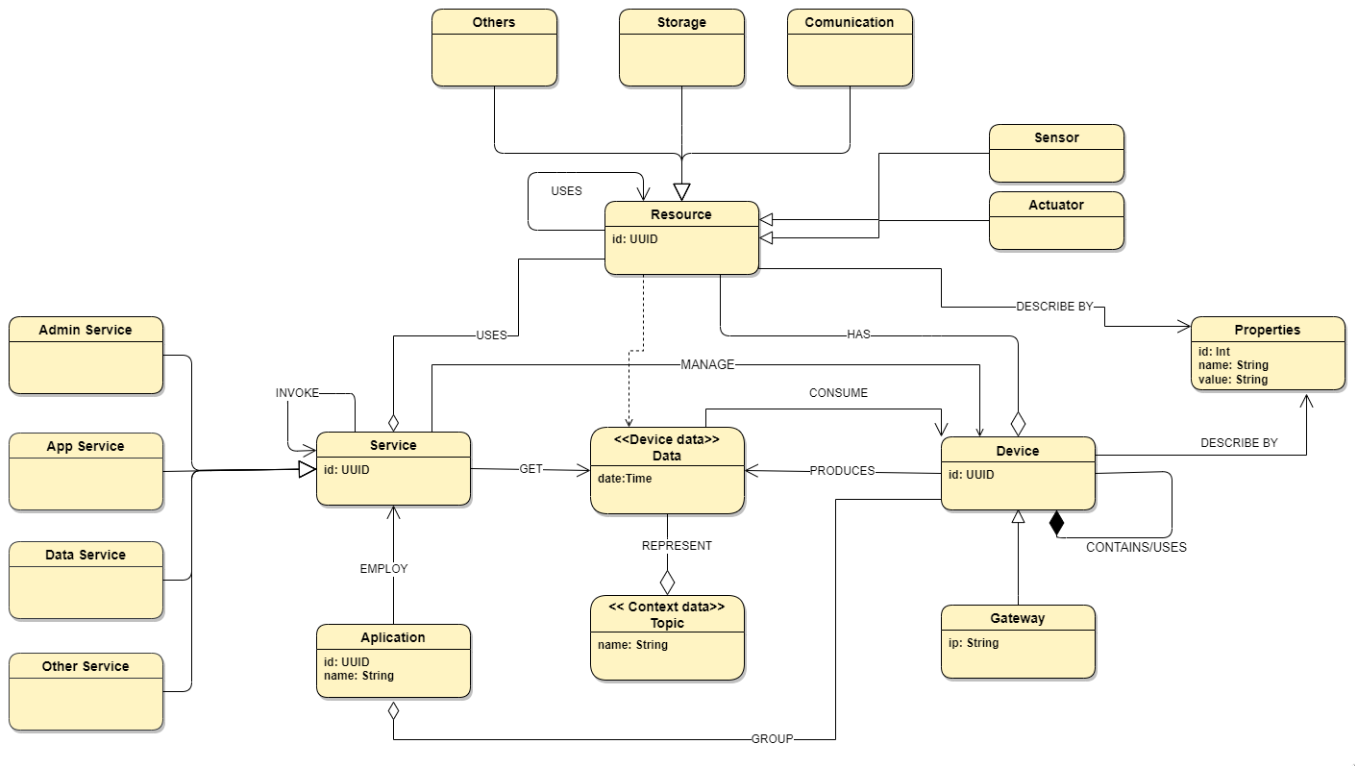
\includegraphics[width=\linewidth]{images/Henrymodelo.png}
\end{figure}

% En este modelo, se presentan todas los componentes que componen a Smart Campus UIS en términos de su arquitectura a un nivel técnico. Ahora, para modelar un Smart Campus a nivel de aplicación, se tomó una versión reducida de este modelo enfocándose en los componentes y a la función que estos cumplen en una ubicación geográfica dada. 

% El basarnos en este modelo nos asegura que se tiene la capacidad de realizar la descripción de un un sistema IoT de Smart Campus en un nivel técnico. Este contiene todos los componentes necesarios para poder modelar

Basarnos en el modelo de la figura \ref{fig:henrymodelo}, nos da la capacidad de describir a un nivel técnico un sistema IoT. Ahora, aunque se podría usar para el desarrollo del proyecto, fue necesario modificarlo con el fin de acercarnos más hacia la descripción de un sistema IoT a nivel de aplicación. 

Lo primero fue el establecer el contexto de los dispositivos. Esto específicamente se refiere al criterio \textit{C2} de la tabla \ref{tab:criterios}, en donde, dada la necesidad de establecer la ubicación geográfica en algunas de las aplicaciones de los Smart Campus, era necesario poder describir los lugares pertenecientes a la aplicación.

Así mismo, se cubre el criterio \textit{C3} cambiando las propiedades del dispositivos de una clase, externa a los dispositivos; a un atributo, interno, el cual le permite a los componentes manejar su propia información en cuanto a los datos que estos manejan. Estas propiedades puede referirse a las entradas que tienen, en el caso de ser actuadores o procesadores de la información; o a los valores que reportan al sistema en el caso de ser sensores.

Partiendo de esto, se planteó el modelo presente en la figura \ref{fig:metamodelo}.

\begin{figure}[H]
    \centering
    \caption{Versión 1 del metamodelo planteado para SCampusADL}
    \label{fig:metamodelo}
    \vspace{2mm}
    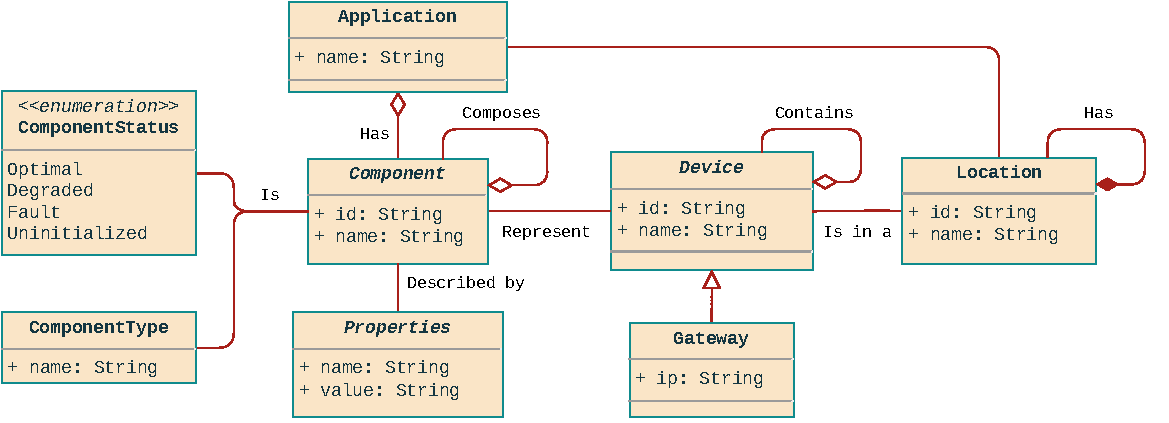
\includegraphics[width=0.8\linewidth]{images/Metamodel B.pdf}
\end{figure}

El enfoque principal del modelo se centra los componentes (\texttt{\textit{Component}}). Estos son las representaciones lógicas, o de software, de las partes de la aplicación. De manera general, pueden ser tanto servicios usados por la aplicación como agregadores de datos, pre-procesadores de datos encargados de transformar los datos recolectados, o incluso los mismos sensores o actuadores que hacen parte del sistema (\textit{\texttt{componentType}}). 

Los componentes pueden ser atómicos, funcionando como entidades independientes, o formar parte de componentes, así como integrarse en componentes aún más grandes. Asimismo, los componentes se describen por una serie de propiedades que hacen referencia tanto al comportamiento al igual que las condiciones las con las cuales se puede evaluar el estado del mismo. 

Estos elementos están presentes en diversos dispositivos (\texttt{\textit{Device}}), los cuales se encargan de la ejecución de partes de la aplicación, o puntos de comunicación entre diversos componentes (\textit{\texttt{Gateway}}). Estos pueden verse como los recursos físicos de la aplicación los cuales se encuentran ubicados en diferentes puntos, o locaciones (\textit{\texttt{location}}), dentro del Campus (\textit{\texttt{Campus}}). 

Lo anterior nombrado hace parte del contexto de la aplicación. Siendo así, estos están relacionados contra la aplicación la cual sirve como un punto de acceso común entre el contexto geográfico y los componentes de software que deben ser manejados.

Finalmente, los estados de los componentes (\textit{\texttt{ComponentStatus}}), reflejan el como estos se encuentran dentro del contexto de la aplicación. Estos pueden variar de óptimo (\textit{\texttt{optimal}}), donde todos los componentes están funcionales según las propiedades establecidas; degradado (\textit{\texttt{degraded}}), donde uno o más de los componentes opcionales está fallado; y fallo (\textit{\texttt{fault}}), que es cuando alguno de los dispositivos obligatorios no está en funcionamiento.

\section{Sintaxis de la notación}

Partiendo de esto, lo siguiente que se realizó fue la definición de la sintaxis de la notación a usar, basados en lo definido por el metamodelo. Para esto, se decidió a usar \texttt{YAML}, un lenguaje de serialización de datos orientado a la legibilidad, reconocido y usado principalmente para la creación de archivos de configuración \cite{YAML2023}. 

La sintaxis, como puede observarse en la figura \ref{fig:rail-base}, se compone de 2 partes: \texttt{locaciones}, para establecer el contexto geográfico de la aplicación; y \texttt{componentes}, con el cual se definen las partes de la aplicación al igual que las propiedades y lugar en el cual deben estar para el funcionamiento de la aplicación.

\begin{figure}[H]
    \centering
    \caption{Diagrama de rail de la sintaxis definida para la notación de SmartCampusADL}
    \label{fig:rail-base}
    \vspace{2mm}
    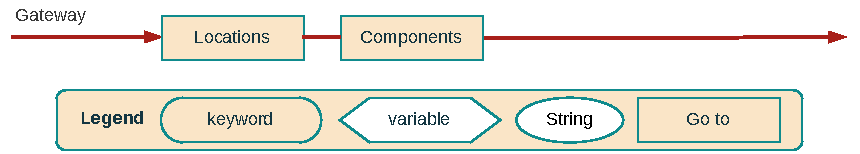
\includegraphics[width=\linewidth]{images/Railroad Base.pdf}
\end{figure}

Para especificar las \texttt{locaciones} dentro del contexto de la aplicación, se definió la sintaxis que puede observarse en la figura \ref{fig:rail-location}. De esta manera, tras especificar la \textit{keyword} \texttt{locations}, se pueden los puntos geográficos necesarios, al igual que las locaciones que lo componen. Así mismo, es posible declarar de manera implícita la ip de la \textit{gateway} que se encuentra en el lugar con el fin de poder establecer el origen de los datos recolectados. 

\begin{figure}[H]
    \centering
    \caption{Diagrama de rail de la sintaxis definida para la notación del contexto geográfico de la aplicación}
    \label{fig:rail-location}
    \vspace{2mm}
    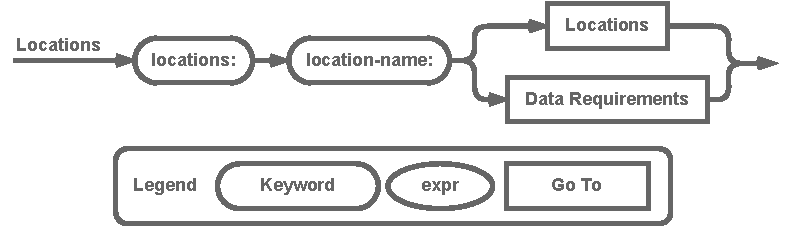
\includegraphics[width=0.8\linewidth]{images/Railroad Locations Alt.pdf}
\end{figure}

Un enfoque similar se aplicó a los componentes. En la figura \ref{fig:rail-components} se presenta la sintaxis a usar para poder definir y ubicar los componentes dentro de la aplicación. De esta forma, se pueden declarar los componentes, al igual que sus propiedades; y algunas de las características que estos deben cumplir para poder ser evaluados dentro del contexto de la aplicación.

\begin{figure}[H]
    \centering
    \caption{Diagrama de rail de la sintaxis definida para la notación de los componentes de la aplicación}
    \label{fig:rail-components}
    \vspace{2mm}
    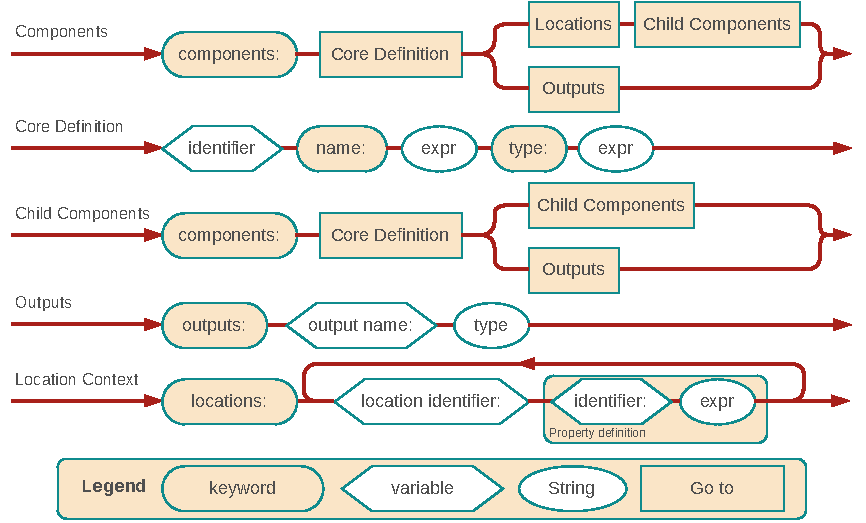
\includegraphics[width=0.8\linewidth]{images/Railroad Components Alt.pdf}
\end{figure}

Al definir esta notación, hemos creado un marco sólido para representar las aplicaciones de Smart Campus UIS. Este enfoque bien definido nos permitirá avanzar en el desarrollo de nuestras funcionalidades de comparación de los modelos, y la implementación de los mecanismos de adaptación a usar. Un ejemplo de como se vería un archivo de notación válido para nuestras necesidades puede encontrarse en el anexo \ref{appendix:example}. 


    
    %   Capítulo 2

    \section{Comparación de Arquitecturas}

\subsection{Conociendo el estado actual}

Con la notación de las arquitecturas objetivo establecidas, al igual que el desarrollo del módulo encargado de la construcción y validación de los archivos de configuración; lo siguiente era la definición del proceso de la comparación entre la arquitectura actual y la arquitectura de referencia. Este proceso, nos permitirá evaluar el estado del sistema y, por consiguiente, establecer las acciones a tomar con el fin de adaptar la arquitectura hacia el estado objetivo establecido.

Esto requiere conocer el estado actual del sistema, al igual que el conocer el estado objetivo. Siendo así, y ya teniendo la posibilidad de declarar las necesidades de la aplicación, lo siguiente es establecer una manera de determinar el estado del sistema. Dado el enfoque hacia los datos recolectados, es necesario el precisar la manera en la que conoceríamos en qué estado se encuentra el sistema.

Partiendo de esto, lo primero era el identificar los puntos de acceso por los cuales podríamos acceder a los datos, en el caso de Smart Campus UIS, como se observa en la figura \ref{fig:ArquitecturaSmartCampus}, hay dos maneras en las que podemos acceder a los datos. La primera, es haciendo consultas a la base de datos en la cual se guardan los registros; la segunda, implica recibir los mensajes que viajan por el bus de datos, sea el de los adaptadores de descripción o el de los dispositivos con el servicio de mensajería , y procesar cada uno de los mensajes.

\begin{figure}[ht]
    \centering
    \caption{Arquitectura del prototipo de Smart Campus definido por }\citeA{msc_henry_2022}
    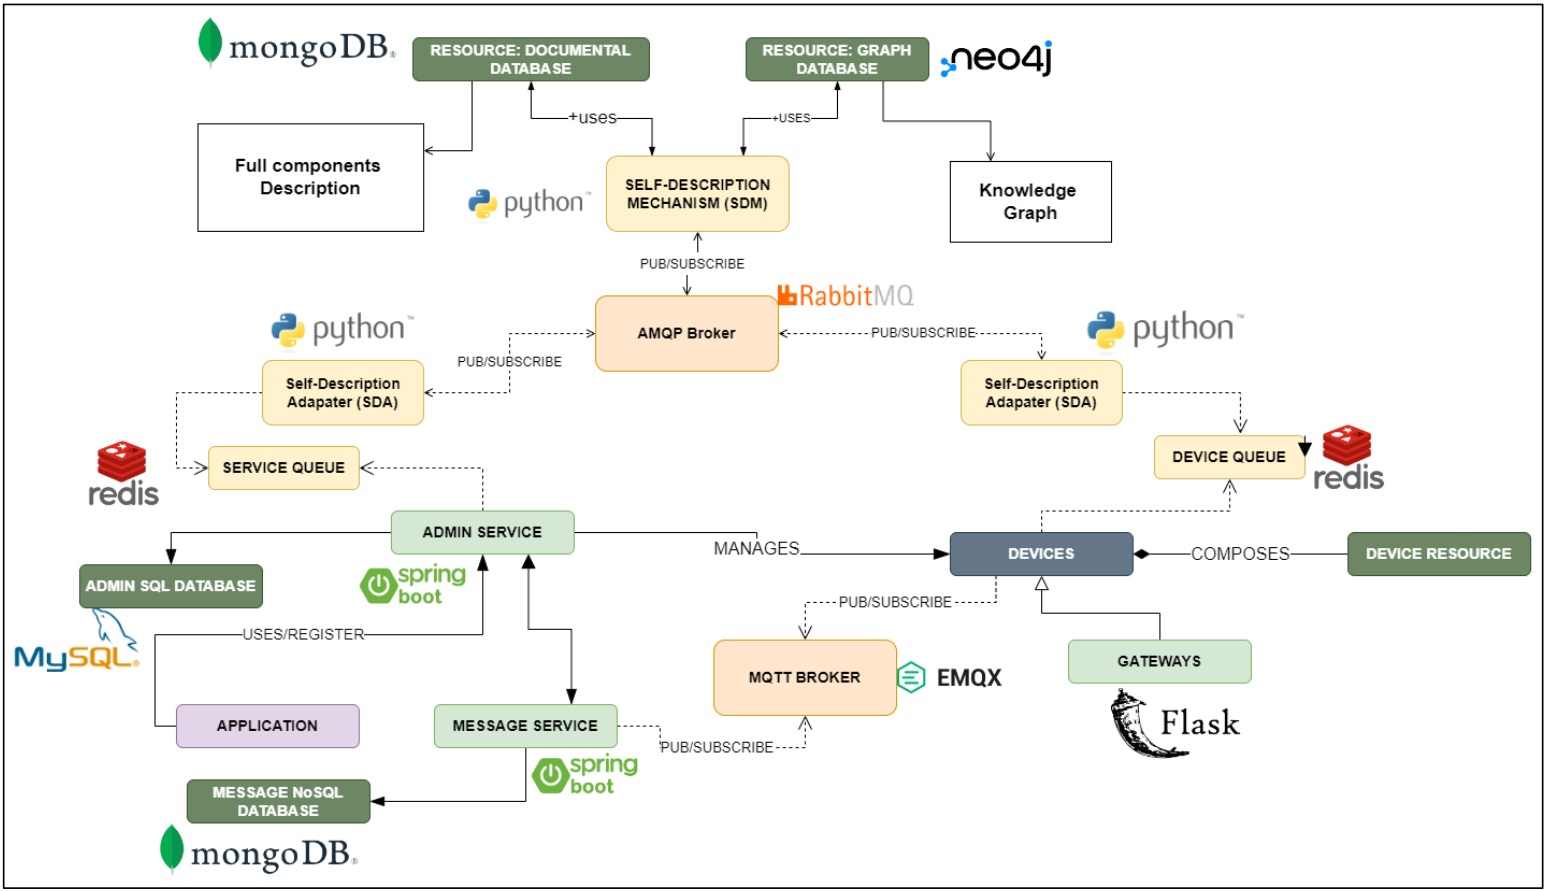
\includegraphics[width=\linewidth]{images/ArquitecturaSmartCampus.png}
    \label{fig:ArquitecturaSmartCampus}
\end{figure}

Ahora, cada una de las maneras de acceder a los datos es viable, y podría permitir la implementación correspondiente para determinar el estado del sistema. Sin embargo, de entre las tres opciones, se escogió el procesamiento de los mensajes de los adaptadores de descripción, enviados por AMQP. Esta decisión se debe a algunas de las ventajas que posee el protocolo sobre la consulta a base de datos. Entre estas destacan la menor latencia en la recuperación y la direccionalidad de datos, comparado con las consultas. 

La primera se refiere a la menor cantidad de saltos de servicios antes de que los datos sean guardados en la base de datos, lo que aumenta el tiempo en el que estos estarán disponibles, sumado a el tiempo ejecución de la consulta. Así mismo, la última refiriéndose a que el protocolo AMQP, gracias a su modelo pub/sub, permite el poder procesar los datos a medida que estos van llegando, y no en intervalos discretos de tiempo, lo cual podría afectar la toma de decisiones.


    
    % \section{Resultados}

    
    % \section{Discusión}

    
    % \section{Conclusiones}


    \newpage
    \bibliography{bibliography.bib}
    
    % \appendix
    
    \appendix
    \newpage
    \section{Apéndices}
    \subsection{Ejemplo de un YAML de una aplicación válida}\label{appendix:example}
    \lstinputlisting[language=YAML]{metamodel/model.yaml}

    % \lstinputlisting[language=YAML]{metamodel/modelV2.yaml}

\end{document}
